\documentclass{article}

%table customization, stack overflow 
\usepackage{array}
\newcolumntype{L}[1]{>{\raggedright\let\newline\\
\arraybackslash\hspace{0pt}}m{#1}}

%figure flaots from http://www.tex.ac.uk/FAQ-figurehere.HTML
\usepackage{float}
\usepackage{color}
\usepackage{tabularx}
\usepackage{enumitem}
\usepackage{graphicx}
\usepackage{booktabs}
\usepackage{url}
\usepackage{hyperref}
\usepackage{fancyhdr}
\pagestyle{fancy}
\begin{document}
\pagenumbering{gobble}
\lhead{Team 6\\ JSTanks\\}
\newpage
\title{JSTanks - Test Report}
\date{December 8, 2016}
\author{Jiahao Li\\LI577\\001416646\and Pavithran Pathmarajah\\PATHMAP\\
001410729 \and Viren Patel\\PATELVH3\\001419057}

\maketitle

\newpage
\pagenumbering{arabic}
\tableofcontents
\newpage
\listoftables

\newpage
\listoffigures

\newpage


\section*{Overview of Document}
This document describes the purposes of the testing done, the scope to which it was done
the tools used, followed by a summarized table to test results linking to the tests themselves,
and closing with a comparison to the original game. 

\section{Revision History}
\begin{table}[H]
\caption{Revision 1}
	\begin{tabularx}{\textwidth}{cXc}
		\toprule
		Date & Developer & Change\\
		\midrule
		December 6&Jiahao Li &Initial Draft \\
		December 6&Pavithran Pathmarajah &Initial Draft\\
		December 6&Viren Patel  &Initial Draft\\
		\midrule
		December 8&Pavithran Pathmarajah &Include Links\\
	\end{tabularx}
\end{table}




\section{General Information}
\subsection{Purpose}
This document is a report outlining the results of the testing, validation and verification process 
that was to be followed by JSTanks after the build process. 



\subsection{Acronyms, Abbreviations, and Symbols}
\begin{figure}[H]
	\centering
	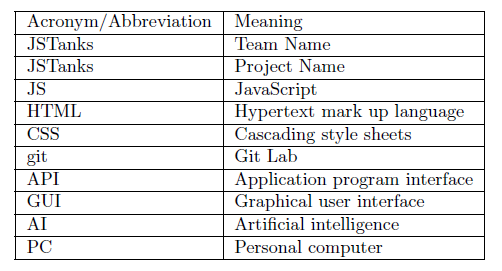
\includegraphics[width=\textwidth]{./Figures/fig1.png}
	\caption{Acronyms}
\end{figure}

\subsection{Scope}
This project was designed to port an existing Java based game to the web
where it will no longer be required to be download and ran locally, instead
it will be able to run in the browser. The tests cover all functionality of the 
game both functional and non-functional.

\section{Tools-Used}
The team used an automated test script as well as Google forms, as tools,
to help in the testing process. The script was used to perform many tests
as fast as possible, as many times as needed to ensure repeatable results
to be certain that the game passed its requirements. Where as google forms
was used as a means to build and distribute a questionnaire, in order to get 
qualitative feedback on the game to check if it passed the non-functional 
requirements set for it.

\subsection{Automated Test Script}
An automated testing script was made., to check for most functional requirements.
The script was able to do many repetitive tests, much quicker then an individual
is able to set up a scenario and run through a test. The script was also able to 
pick out specific calls as they occurred in order to see if the correct result occurred.

\subsubsection{Load In Scripts}
\begin{itemize}  
\item Each test ran is located in a separate test file labelled testN, where N is the test number.
	This script dynamically tries to load in test scripts numbered form 0 to 100, to allow for 
	tests to be added on the fly.
\item No other tests will begin until this script loads in the tests, if the script is unable to find the
	scripts then their is an error and no tests are ran.

\end{itemize}

\subsubsection{Page Load}
\begin{itemize}  
\item Ensures that all HTML pages and subsequent scripts on each page load up, this is
	checked by the script binding to the webpage and waiting for loading of files to 
	complete. Once all files are loaded for a specified page the script moves onto the
	next page.
\item If any one page takes more than two seconds to load then the test fails.
\end{itemize}

\subsubsection{Menu Functionality}
\begin{itemize}  
\item Runs through all menus on every page and checks that Javascript functions are 
	linked and function correctly.
\item If any one javascript call on a menu does not work, or throws an error, the whole 
	test fails
\end{itemize}

\subsubsection{Board Boundaries}
\begin{itemize}  
\item Creates a blank board and places a user tank in one corner, then tries to move the
	tank 20 times in one direction, (Trying to throw and error on a 15 x 15 board).
\item The game then places wall objects on the board in a cross pattern, then runs the same 
	test failing if the tank tile moves to a spot where a wall object is located.  
\item The script then replaces the wall objects with steel walls and tries again.
\item The script then replaces the steel wall object with home bases tries again,
\item If the tank entity moves to  a location that it should not the whole test fails. 
	The check is done via a script cross checking the x and y position of the tank with
	the board.
\end{itemize}

\subsubsection{Game Pause}
\begin{itemize}  
\item Checks the pause and unpause features works correctly
\item When the game is paused a script runs code and takes snapshots of the board array
	checking if the board changes at all while paused. 
\item The script mimics key press of 'p' to pause 
\item The script then replaces the steel wall object with home bases tries again,
\item The script then mimics the continue button being pressed as well
\item If the board updates while paused or the continue feature or 'p' key
	do not work correctly the test fails.
\end{itemize}

\subsubsection{Ai Randomness}
\begin{itemize}  
\item Checks the AI functions by starting a new game and removing all tanks
	but one AI tank.
\item If over the course of two seconds the tank has a net displacement of 2 tiles
	it passes.
\end{itemize}

\subsubsection{Projectiles}
\begin{itemize}  
\item Checks that the projectile fire function fires a projectile
\item Checks that when a projectile hits a wall it takes damage
\item Checks that when a projectile hits a steel wall it takes damage
\item Checks that when a projectile hits a base it takes damage
\item Checks that when a projectile hits a tank it takes damage
\item Checks that a projectile is dequeued when it hits something
	or goes off screen
\item Does this by binding to multiple functions in the game javascript
\end{itemize}

\subsubsection{Player Tank}
\begin{itemize}  
\item Checks that user input works correctly, does so by triggering 
	keyboard events.
\item The script cross checks the old tank position with new positions 
	on the board, to check if it moved accordingly.
\item The script checks that the fire command had worked correctly by 
	placing a wall where the tank should, be and seeing if it was 
	damaged.
\end{itemize}

\subsubsection{Game End}
\begin{itemize}  
\item Checks the game ends when the home base is destroyed.
\item  Checks with multiple home bases.
\item Checks the game ends when the AI is killed.
\item  Checks with multiple AI.
\item Checks if the game ends when the player tank is destroyed.
\item Test is done by script binding to the end game call, if any scenario
	does not end the game then the test is failed.
\end{itemize}

 \subsubsection {Link to Test Script}
\hspace{10 mm}
{\color{blue}   \href{http://pavipath.com/JSTanks/Testing/Test.html}{JSTank Automated Tester}}


\subsection{Questionnaire}
A questionnaire was issued via google forms to ensure non-functional requirements 
were met through the process of performing a qualitative analysis to determine 
whether the requirements were met. The questionnaire issued was 7 pages long 
and was filled by 8 people. The links below will forward you to a PDF of the 
questionnaire and the google form itself.

 \subsubsection {Link to Questionnaire}
\hspace{10 mm}
{\color{blue}   \href{http://sl.pavipath.com/2gJSSurvey}{Google Form - Questionnaire}}
  
\subsubsection {PDF of Questionnaire}
\hspace{10 mm}
{\color{blue}  \href{file:///../../ReferenceMaterial/questionnaire.pdf}{PDF of Questionnaire}}



\section{Test Summary}
The game has passed all the tests designed by the team in order to check that it meets all 
functional and non-functional requirements. These tests were done via automated testing 
using a custom script, manual testing by the team as-well as by issuing a questionnaire 
and using feedback to determine if the game succeeded or failed. Below are a series of
tables, listing the requirement tests status and last test date (the requirements link to the 
full requirements located further down this document).    

\subsection{Functional Tests}
%game
\begin{table}[H]
\caption{Functional Requirements}
	\begin{tabularx}{\textwidth}{| c | l | X | l |}
	\toprule
	Test \#& Team Member &Comments &Date\\
	\midrule
	\hyperref[sec:3.1.1]{3.1.1}& Automated Script  & SUCCESSFUL & 12\textbackslash
	6\textbackslash2016\\
	\hyperref[sec:3.1.2]{3.1.2}& Automated Script  & Loads HomePage & 12\textbackslash
	6\textbackslash2016\\
	\hyperref[sec:3.1.3]{3.1.3}& Automated Script  & SUCCESSFUL & 12\textbackslash
	6\textbackslash2016\\
	\hyperref[sec:3.1.4]{3.1.4}& Automated Script  & SUCCESSFUL & 12\textbackslash
	6\textbackslash2016\\
	\hyperref[sec:3.1.5]{3.1.5}& Automated Script  & SUCCESSFUL & 12\textbackslash
	6\textbackslash2016\\
	\hyperref[sec:3.1.6]{3.1.6}& Automated Script  & Moves Accordingly & 12\textbackslash
	6\textbackslash2016\\
	\hyperref[sec:3.1.7]{3.1.7}& Automated Script  & SUCCESSFUL & 12\textbackslash
	6\textbackslash2016\\
	\hyperref[sec:3.1.8]{3.1.8}& Automated Script  & SUCCESSFUL & 12\textbackslash
	6\textbackslash2016\\
	\hyperref[sec:3.1.9]{3.1.9}& Automated Script  & SUCCESSFUL & 12\textbackslash
	6\textbackslash2016\\
	\hyperref[sec:3.1.10]{3.1.10}& Automated Script  & SUCCESSFUL & 12\textbackslash
	6\textbackslash2016\\
	\hyperref[sec:3.1.11]{3.1.11}& Automated Script  & SUCCESSFUL & 12\textbackslash
	6\textbackslash2016\\
	\hyperref[sec:3.1.12]{3.1.12}& Automated Script  & SUCCESSFUL & 12\textbackslash
	6\textbackslash2016\\
	\hyperref[sec:3.1.3]{3.1.13}& Automated Script  & SUCCESSFUL & 12\textbackslash
	6\textbackslash2016\\
	\hyperref[sec:3.1.4]{3.1.14}& Automated Script  & SUCCESSFUL & 12\textbackslash
	6\textbackslash2016\\
	\hyperref[sec:3.1.5]{3.1.15}& Automated Script  & SUCCESSFUL & 12\textbackslash
	6\textbackslash2016\\
	\hyperref[sec:3.1.16]{3.1.16}& Automated Script  & SUCCESSFUL & 12\textbackslash
	6\textbackslash2016\\
	\hyperref[sec:3.1.17]{3.1.17}& Automated Script  & SUCCESSFUL & 12\textbackslash
	6\textbackslash2016\\
	\hyperref[sec:3.1.18]{3.1.18}& Automated Script  & SUCCESSFUL & 12\textbackslash
	6\textbackslash2016\\
	\hyperref[sec:3.1.19]{3.1.19}& Automated Script  & SUCCESSFUL & 12\textbackslash
	6\textbackslash2016\\
	\hyperref[sec:3.1.20]{3.1.20}& Automated Script  & SUCCESSFUL & 12\textbackslash
	6\textbackslash2016\\
	\hyperref[sec:3.1.21]{3.1.21}& Automated Script  & SUCCESSFUL & 12\textbackslash
	6\textbackslash2016\\
	\hyperref[sec:3.1.22]{3.1.22}& Automated Script  & SUCCESSFUL & 12\textbackslash
	6\textbackslash2016\\
	\hyperref[sec:3.1.23]{3.1.23}& Automated Script  & SUCCESSFUL & 12\textbackslash
	6\textbackslash2016\\
	\hyperref[sec:3.1.24]{3.1.24}& Automated Script  & SUCCESSFUL & 12\textbackslash
	6\textbackslash2016\\
	\hyperref[sec:3.1.25]{3.1.25}& Automated Script  & SUCCESSFUL & 12\textbackslash
	6\textbackslash2016\\
	\hyperref[sec:3.1.26]{3.1.26}& Automated Script  & SUCCESSFUL & 12\textbackslash
	6\textbackslash2016\\
	\hyperref[sec:3.1.27]{3.1.27}& Automated Script  & SUCCESSFUL & 12\textbackslash
	6\textbackslash2016\\
	\hyperref[sec:3.1.28]{3.1.28}& Automated Script  & SUCCESSFUL & 12\textbackslash
	6\textbackslash2016\\
		\bottomrule
	\end{tabularx}
\end{table}
\subsection{Unit Tests}
\begin{table}[H]
\caption{Unit Tests}
	\begin{tabularx}{\textwidth}{| c | l | X | l |}
	\toprule
	Test \#& Team Member &Comments &Date\\
	\midrule
	\hyperref[sec:3.2.1]{3.2.1}& Automated Script  & SUCCESSFUL & 12\textbackslash
	6\textbackslash2016\\
	\hyperref[sec:3.2.2]{3.2.2}& Automated Script  & SUCCESSFUL & 12\textbackslash
	6\textbackslash2016\\
	\hyperref[sec:3.2.3]{3.2.3}& Automated Script  & SUCCESSFUL & 12\textbackslash
	6\textbackslash2016\\
	\hyperref[sec:3.2.4]{3.2.4}& Automated Script  & Wall Visible & 12\textbackslash
	6\textbackslash2016\\
	\hyperref[sec:3.2.5]{3.2.5}& Automated Script  & Steel Wall Visible & 12\textbackslash
	6\textbackslash2016\\
	\hyperref[sec:3.2.6]{3.2.6}& Automated Script  & Home Base Visible & 12\textbackslash
	6\textbackslash2016\\
	\hyperref[sec:3.2.7]{3.2.7}& Automated Script  & SUCCESSFUL & 12\textbackslash
	6\textbackslash2016\\
	\hyperref[sec:3.2.8]{3.2.8}& Automated Script  & SUCCESSFUL & 12\textbackslash
	6\textbackslash2016\\
	\hyperref[sec:3.2.9]{3.2.9}& Automated Script  & SUCCESSFUL & 12\textbackslash
	6\textbackslash2016\\
	\hyperref[sec:3.2.10]{3.2.10}& Automated Script  & SUCCESSFUL & 12\textbackslash
	6\textbackslash2016\\
	\hyperref[sec:3.2.11]{3.2.11}& Automated Script  & SUCCESSFUL & 12\textbackslash
	6\textbackslash2016\\
	\hyperref[sec:3.2.12]{3.2.12}& Automated Script  & SUCCESSFUL & 12\textbackslash
	6\textbackslash2016\\
	\hyperref[sec:3.2.13]{3.2.13}& Automated Script  & SUCCESSFUL & 12\textbackslash
	6\textbackslash2016\\
	\hyperref[sec:3.2.14]{3.2.14}& Automated Script  & Tank Visible & 12\textbackslash
	6\textbackslash2016\\
	\hyperref[sec:3.2.15]{3.2.15}& Automated Script  & SUCCESSFUL & 12\textbackslash
	6\textbackslash2016\\
	\hyperref[sec:3.2.16]{3.2.16}& Automated Script  & SUCCESSFUL & 12\textbackslash
	6\textbackslash2016\\
	
		\bottomrule
	\end{tabularx}
\end{table}
\subsection{Non-Functional Tests}
\begin{table}[H]
\caption{non-Functional Tests}
	\begin{tabularx}{\textwidth}{| c | l | X | l |}
	\toprule
	Test \#& Team Member &Comments &Date\\
	\midrule
	\hyperref[sec:4.1]{4.1}& Automated Script  & SUCCESSFUL & 12\textbackslash
	6\textbackslash2016\\
	\hyperref[sec:4.2]{4.2}& Automated Script  & SUCCESSFUL & 12\textbackslash
	6\textbackslash2016\\
	\hyperref[sec:4.3]{4.3}& Automated Script  & SUCCESSFUL & 12\textbackslash
	6\textbackslash2016\\
	\hyperref[sec:4.4]{4.4}& Automated Script  & SUCCESSFUL & 12\textbackslash
	6\textbackslash2016\\
	\hyperref[sec:4.5]{4.5}& Automated Script  & SUCCESSFUL & 12\textbackslash
	6\textbackslash2016\\
	\hyperref[sec:4.6]{4.6}& Automated Script  & SUCCESSFUL & 12\textbackslash
	6\textbackslash2016\\
	\hyperref[sec:4.7]{4.7}& Automated Script  & SUCCESSFUL & 12\textbackslash
	6\textbackslash2016\\
	
		\bottomrule
	\end{tabularx}
\end{table}


\section{Tests Performed}
\subsection{Tests for Functional Requirements}
\subsubsection{HTML file test}
\label{sec:3.1.1}
Name:  Loading the game \newline
Description: Test if the game dependencies load in browser
\newline
Type: Unit test (dynamic, automatic, black box) \newline
Initial State:  Testing Script Loaded in \newline
Input: Click the Run Script button \newline
Output: Script is successful, Loads Dependencies \newline
Pass:  All files are able to be loaded up. \newline
\newline Status: PASSED

\subsubsection{Standby state test}
\label{sec:3.1.2}
Name:  Standby state\newline
Description: Test if the game automatically runs or waits
for user initialization. \newline
Type: Unit test (static, manual, black box) \newline
Initial State: A new browser \newline
Input: Go to home page of game \newline
Output: The home page of the game \newline
Pass: The browser remains on the home page. \newline
\newline Status: PASSED

\subsubsection{The game section of the menu test}
\label{sec:3.1.3}
Name: Menu of game section\newline
Description: Test if the sub menu of new game section which has choices of 
level selection and map selection show up.
\newline
Type: Unit test (dynamic, automatic, black box) \newline
Initial State: Menu in the standby state \newline
Input: Script selects new game \newline
Output:  Menu Tests successfully  \newline
Pass: The sub menu with choice of starting a new game and quit. \newline
\newline Status: PASSED

\subsubsection{The pause section of the menu test}
\label{sec:3.1.4}
Name:  Menu representation\newline
Description: check if the menu contains Home Page/Continue/
Instructions/New Game/Quit \newline
Type: Unit test (dynamic, automatic, black box) \newline
Initial State: A new browser \newline
Input: Click the Run Script button \newline
Output: Menu Tests successfully \newline
Pass: The menu with five sections is represented in the standby state. \newline
\newline Status: PASSED

\subsubsection{The level section of the menu test}
\label{sec:3.1.5}
Name:  Menu of level\newline
Description: Test if the sub menu of level section which has choices of level 
1, level 2, and level 3 shows up when the level section is clicked. \newline
Type: Unit test (dynamic, automatic, black box) \newline
Initial State: Menu in the new game state \newline
Input: Script runs through levels\newline
Output: New Game Success\newline
Pass: The sub menu with choice of level 1, level 2, level 3, level 4 and level 5. \newline
\newline Status: PASSED

\subsubsection{Game start test}
\label{sec:3.1.6}
Name:  Start the game\newline
Description: Test if the game shall be reset and start when [starting a new 
game] is clicked. \newline
Type: Unit test (dynamic, automatic, black box) \newline
Initial State:  The sub menu of the game section \newline
Input: Click the choice of starting a new game \newline
Output: New Game Success\newline
Pass: The standby state of the game with all objects on their initial position 
on the map. \newline
\newline Status: PASSED

\subsubsection{Game quit test}
\label{sec:3.1.7}
Name:  Quit the game\newline
Description: Test if the game comes to ends and the user is redirected to
 the repo if the quit is clicked \newline
Type: Unit test (dynamic, automatic, black box) \newline
Initial State:  The running state of the game \newline
Input: Click the Quit option\newline
Output: Menu Tests successfully \newline
Pass: The game is redirected to the gitlab repository.  \newline
\newline Status: PASSED

\subsubsection{Game pause test}
\label{sec:3.1.8}
Name:  Pause the game\newline
Description: Test if the game comes to the pause state when the letter 'p' is 
pressed on the keybaord. \newline
Type: Unit test (dynamic, automatic, black box) \newline
Initial State: The running state of the game \newline
Input: Script triggers a keyboard event 'p'\newline
Output: The game pauses and the pause menu shows up \newline
Pass: The game comes to a pause state. Game content freezes and 
stays in the temporal positions whilst the Pause menu is overlayed . \newline
\newline Status: PASSED

\subsubsection{Game continue test 0}
\label{sec:3.1.9}
Name:  Continue the game\newline
Description: Test if the game comes back to the running state state when the letter 'p' is 
pressed on the keyboard. \newline
Type: Unit test (dynamic, automatic, black box) \newline
Initial State: The pause state of the game\newline
Input: Script triggers a keyboard event 'p'\newline
Output: The game resumes \newline
Pass: All stuff frozen in the pause state are activated and back into the 
routine. \newline
\newline Status: PASSED

\subsubsection{Game continue test 1}
\label{sec:3.1.10}
Name:  Continue the game in the running state\newline
Description: Test if there is any effect on the game when the choice of 
continue is clicked in the running state. \newline
Type: Unit test (dynamic, automatic, black box) \newline
Initial State: The running state of the game \newline
Input: Script triggers a click on continue\newline
Output: No effect \newline
Pass: No effect on the running state. \newline
\newline Status: PASSED

\subsubsection{AI test}
\label{sec:3.1.11}
Name:  The routine of AI\newline
Description: Test if the AI controls tanks to move and fire randomly. \newline
Type: Unit test (dynamic, automated, white box) \newline
Initial State: Single AI in centre of empty game board \newline
Input: The script is run \newline
Output: Ai Test succesful \newline
Pass: The script tracks the AI movement over the course of 2 seconds,
and if the AI has a net travel of more then 2 tiles, then it passes.
 \newline
 \newline Status: PASSED

\subsubsection{Level test}
\label{sec:3.1.12}
Name:  Levels of the game\newline
Description: Test if the moving speed of tanks controlled by the AI change 
when level 1, level 2, level 3, level 4 or level 5 is clicked. \newline
Type: Unit test (dynamic, automated, black box) \newline
Initial State:  The running state of the game \newline
Input:The script is run\newline
Output: New game test is succesful\newline
Pass: The script checks the AI movement delay value of each game, 
and if they correspond high to low with the level chosen, then it passes.
 \newline
 \newline Status: PASSED

\subsubsection{Default level test}
\label{sec:3.1.13}
Name:  The default level of the game\newline
Description: Test if level one is chosen if no level is selected. Since the
game pareses the level form the URL.  \newline
Type: Unit test (static, automated, white box) \newline
Initial State: The new browser windwo \newline
Input: Script redirects to the /JSTanks.Html page directly \newline
Output: The game starts with tanks controlled by the AI moving in the lowest 
speed\newline
Pass: The script checks the AI movement delay value is at the lowest normal
 value it can be.\newline
 \newline Status: PASSED

\subsubsection{Instructions test}
\label{sec:3.1.14}
Name:  The Instructions of the game\newline
Description: Test if The window with the Instructions of the game in it pops up 
when the section of Instructions is clicked. \newline
Type: Unit test (dynamic, automated, black box) \newline
Initial State: New browser window \newline
Input: Script opens instructions page\newline
Output: Pages Section of script is succseful\newline
Pass:  The instructions modal opens with the instructions displayed.  \newline
\newline Status: PASSED

\subsubsection{Tank test}
\label{sec:3.1.15}
Name:  The movement of the tank controlled by the user\newline
Description: Test if the tank controlled by the user moves left, right, up or 
down when the left, right, up or down key on the keyboard is pressed and
fires when the f key is pressed. \newline
Type: Unit test (dynamic, automated, black box) \newline
Initial State:  The running state of the game \newline
Input: Script triggers left, right, up, down or 'f' keyboard events\newline
Output: Script tank is succesful\newline
Pass: The tank moves accordingly with the key board input and 
fires when "F" is pressed. \newline
\newline Status: PASSED

\subsubsection{Continuous movement test}
\label{sec:3.1.16}
Name:  The continuous movement of the tank controlled by the user\newline
Description: Test if the tank controlled by the user keeps moving in the 
direction of left, right, up or down when the left, right, up or down key on 
the keyboard is held. \newline
Type: Unit test (dynamic, manual, black box) \newline
Initial State:  The running state of the game \newline
Input: Hold the left, right, up or down key on the keyboard\newline
Output: The continuous movement of the tank controlled by the user\newline
Pass:  The tank keeps moving in the correct direction according to the key 
held by the user until the user release the key. \newline
\newline Status: PASSED

\subsubsection{Bullet launch test}
\label{sec:3.1.17}
Name:  Launch the bullet\newline
Description: Test if a bullet is correctly launched by the fire commands \newline
Type: Unit test (dynamic, automatic, black box) \newline
Initial State: Blank game Screen\newline
Input: Script calls the fire functionality of the game\newline
Output: Script projectiles is successful  \newline
Pass: A bullet is fired.\newline
\newline Status: PASSED

\subsubsection{Bullet movement test}
\label{sec:3.1.18}
Name:  The movement the bullet\newline
Description: Test if the bullet keep moving in the same direction after being 
launched. \newline
Type: Unit test (dynamic, automated, black box) \newline
Initial State:  The bullet is launched \newline
Input: --\newline
Output: Script projectiles is successful  \newline
Pass: A bullet moves continuously in the same direction.\newline
\newline Status: PASSED

\subsubsection{Bullet disappearance test}
\label{sec:3.1.19}
Name:  The bullet disappearance \newline
Description: Test if the bullet disappears when it hits the tank, wall, steel,
 home base or the boundary of the map. \newline
Type: Unit test (dynamic, automated, black box) \newline
Initial State:  The bullet is moving in a specific direction\newline
Input: --\newline
Output: Script projectiles is successful  \newline
Pass: The bullet disappears when it hits the tank, wall, steel, home base or 
the boundary of the map. \newline
\newline Status: PASSED

\subsubsection{Wall hit test}
\label{sec:3.1.20}
Name:  The wall hit by the bullet\newline
Description: Test if the wall disappears when it is hit by the bullet. \newline
Type: Unit test (dynamic, automated, black box) \newline
Initial State:  Bullet fired toward a wall \newline
Input: --\newline
Output: Script projectiles is successful  \newline
Pass:  The wall disappears immediately when it is hit by the bullet. \newline
\newline Status: PASSED

\subsubsection{Steel hit test 0}
\label{sec:3.1.21}
Name:  The steel hit by the bullet twice\newline
Description: Test if the steel stays the same when it is hit by the bullet 
twice. \newline
Type: Unit test (dynamic, automated, black box) \newline
Initial State:  Bullet fired toward a steel wall \newline
Input: --\newline
Output: Script projectiles is successful  \newline
Pass:  The steel tile remains on screen but its strength is decreased. \newline
\newline Status: PASSED


\subsubsection{Enemy tanks hit test}
\label{sec:3.1.22}
Name:  The tank controlled by the AI hit by the bullet\newline
Description: Test if the tank controlled by the AI disappears when it is hit 
by the bullet. \newline
Type: Unit test (dynamic, automated, black box) \newline
Initial State:  The tank controlled by the AI is on screen \newline
Input: Bullets fired at tank\newline
Output: Script end game is succesful\newline
Pass: The tank controlled by the AI disappears when it is hit by the bullets.
\newline
\newline Status: PASSED


\subsubsection{Home base hit test 0}
\label{sec:3.1.23}
Name:  The home base hit by the bullet for first four times\newline
Description: Test if the home base stays the same when it is hit by the bullet 
for first four times. \newline
Type: Unit test (dynamic, automated, black box) \newline
Initial State:  The home base is on screen \newline
Input: Bullets fired at base\newline
Output: Script projectiles is successful  \newline
Pass:  The home base stays the same when it is hit by the bullet for the first 
four times. \newline
\newline Status: PASSED


\subsubsection{Home base hit test 1}
\label{sec:3.1.24}
Name: The home base hit by the bullet at the fifth time\newline
Description: Test if the home base disappears when it is hit by the bullet  at 
the fifth time. \newline
Type: Unit test (dynamic, automated, black box) \newline
Initial State:  The damaged home base is on screen \newline
Input: Bullets fired at tank\newline
Output: Script end game is successful\newline
Pass: The home base disappears when it is hit by the bullet a fifth 
time. \newline
\newline Status: PASSED

\subsubsection{User tank hit test 0}
\label{sec:3.1.25}
Name: The tank controlled by the user hit by the bullet for the first time
\newline
Description: Test if the tank controlled by the user stays the same when it is 
hit by the first bullet. \newline
Type: Unit test (dynamic, automated, black box) \newline
Initial State:  The tank controlled by the user is on screen \newline
Input: bullets fired at tank\newline
Output: Script projectiles is successful  \newline
Pass: The tank controlled by the user stays the same when it is hit by the 
bullet for the first four times. \newline
\newline Status: PASSED

\subsubsection{User tank hit test 1}
\label{sec:3.1.26}
Name:  The tank controlled by the user hit by the bullet at the fifth time
\newline
Description: Test if the tank controlled by the user disappears when it is hit 
by the bullet at the fifth time. \newline
Type: Unit test (dynamic, automated, black box) \newline
Initial State:  The damaged tank controlled by the user is on screen
 \newline
Input: Bullets fired at tank\newline
Output: Script end game is successful\newline
Pass: The tank controlled by the user disappears when it is hit by the bullet 
a fifth time. \newline
\newline Status: PASSED

\subsubsection{Game over test 0}
\label{sec:3.1.27}
Name:  The player tank is destroyed\newline
Description: Test if the game comes to the end state when the tank controlled 
by the user disappears. \newline
Type: Unit test (dynamic, automated, black box) \newline
Initial State:  The tank controlled by the user disappears\newline
Input: bullets fired at tank\newline
Output: Script end game is successful\newline
Pass:  The player tank is destroyed and the game enters an End state. \newline
\newline Status: PASSED

\subsubsection{Game over test 1}
\label{sec:3.1.28}
Name:  The home base is destroyed\newline
Description: Test if the game comes to the end state when the home base 
disappears. \newline
Type: Unit test (dynamic, automated, black box) \newline
Initial State:  The damaged home base is on screen \newline
Input: Bullets fired at base\newline
Output: Script end game is successful\newline
Pass:  The base is destroyed and the game enters an End state \newline
\newline Status: PASSED


\subsection{Unit testing for internal functions}

\subsubsection{Wall type test}
\label{sec:3.2.1}
Name:  Ask for the type of the wall\newline
Description: Test if the program returns the type of the wall when you ask for 
it. \newline
Type: Unit test (dynamic, automated, white box) \newline
Initial State:  Barriers on screen made of specified wall typel \newline
Input: wall.type()\newline
Output: "BARRIER"  \newline
Pass:   The program returns the type "BARRIER" when wall.type() is called. 
\newline
\newline Status: PASSED

\subsubsection{Steel type test}
\label{sec:3.2.2}
Name:  Ask for the type of the steel\newline
Description: Test if the program returns the type of the steel when you ask for 
it. \newline
Type: Unit test (dynamic, automated, white box) \newline
Initial State:  Barriers on screen made of type steel \newline
Input: steel.type()\newline
Output: "BARRIER"  \newline
Pass:  The program returns the type "BARRIER" when wall.type() is called. 
\newline
\newline Status: PASSED

\subsubsection{Home base type test}
\label{sec:3.2.3}
Name:  Ask for the type of the home base\newline
Description: Test if the program returns the type of the home base when you ask
 for it. \newline
Type: Unit test (dynamic, automated, white box) \newline
Initial State:  Barriers on screen made of type home base \newline
Input: homebase.type()\newline
Output:""BARRIER \newline
Pass:  The program returns the type "BARRIER" when wall.type() is called. 
\newline
\newline Status: PASSED

\subsubsection{Wall draw test}
\label{sec:3.2.4}
Name:  Draw the wall on the game board\newline
Description: Test if the image of the wall shows up on the position we set on
 the game board in the right size when we call this function. \newline
Type: Unit test (dynamic, manual, white box) \newline
Initial State:  The game board with no image on the position (startX,startY) 
\newline
Input: wall.draw(canvas,startX,startY,tileSize,t)\newline
Output: The image of the wall shows up on the position (startX,startY) of the 
game board\newline
Pass:  The image of the wall shows up on the position (startX,startY) of the 
game board in the tileSize. \newline
\newline Status: PASSED

\subsubsection{Steel draw test}
\label{sec:3.2.5}
Name:  Draw the steel on the game board\newline
Description: Test if the image of the steel shows up on the position we set on 
the game board in the right size when we call this function. \newline
Type: Unit test (dynamic, manual, white box) \newline
Initial State:  The game board with no image on the position (startX,startY) 
\newline
Input: steel.draw(canvas,startX,startY,tileSize,t)\newline
Output: The image of the steel shows up on the position (startX,startY) of the
 game board\newline
Pass:  The image of the steel shows up on the position (startX,startY) of the 
game board in the tileSize. \newline
\newline Status: PASSED

\subsubsection{Home base draw test}
\label{sec:3.2.6}
Name:  Draw the home base on the game board\newline
Description: Test if the image of the home base shows up on the position we 
set on the game board in the right size when we call this function. \newline
Type: Unit test (dynamic, manual, white box) \newline
Initial State:  The game board with no image on the position (startX,startY) 
\newline
Input: homebase.draw(canvas,startX,startY,tileSize,t)\newline
Output: The image of the home base shows up on the position (startX,startY) of
 the game board\newline
Pass:  The image of the home base shows up on the position (startX,startY) of 
the game board in the tileSize. \newline
\newline Status: PASSED

\subsubsection{Wall hit test}
\label{sec:3.2.7}
Name:  Hit the wall\newline
Description: Test if the program decreases the points of strength of the wall 
after it has been hit. \newline
Type: Unit test (dynamic, automated, white box) \newline
Initial State:  Wall on screen\newline
Input: projectile hits wall\newline
Output: Script projectiles is successful  \newline
Pass:  The wall is destroyed and thus disappears from the game board.
\newline
\newline Status: PASSED

\subsubsection{Steel hit test}
\label{sec:3.2.8}
Name:  Hit the steel\newline
Description: Test if the program decreases the points of strength of the steel 
after it has been hit. \newline
Type: Unit test (dynamic, automated, white box) \newline
Initial State:  Steel Walll on screen\newline
Input: projectile hits steel wall\newline
Output: Script projectiles is successful  \newline
Pass:  One point of strength of the steel wall is decreased after a hit. 
\newline
\newline Status: PASSED

\subsubsection{Home base hit test}
\label{sec:3.2.9}
Name:  Hit the home base\newline
Description: Test if the program decreases the points of strength of the home 
base after it has been hit. \newline
Type: Unit test (dynamic, automated, white box) \newline
Initial State:  home base on screen\newline
Input: projectile hits base\newline
Output: Script projectiles is successful  \newline
Pass:  One point of strength of the home base is decreased after a hit. 
\newline
\newline Status: PASSED

\subsubsection{Wall health get test}
\label{sec:3.2.10}
Name:  Get health of the wall\newline
Description: Test if the program returns the remaining points of strength of 
the wall after calling this function. \newline
Type: Unit test (dynamic, automated, white box) \newline
Initial State:  wall on screen\newline
Input: projectile hits wall\newline
Output: Script projectiles is successful  \newline
Pass:  Return the remaining points of strength of the wall after calling this 
function. \newline
\newline Status: PASSED

\subsubsection{Steel health get test}
\label{sec:3.2.11}
Name:  Get health of the steel\newline
Description: Test if the program return the remaining points of strength of 
the steel wall after calling this function. \newline
Type: Unit test (dynamic, automated, white box) \newline
Initial State:  steel wall on screen\newline
Input: projectile hits steel wall\newline
Output: Script projectiles is successful  \newline
Pass:  Return the remaining points of strength of the steel wall after calling this 
function. \newline
\newline Status: PASSED

\subsubsection{Home base health get test}
\label{sec:3.2.12}
Name:  Get health of the home base\newline
Description: Test if the program return the remaining points of strength of the
home base after calling this function. \newline
Type: Unit test (dynamic, automated, white box) \newline
Initial State:  home base on screen\newline
Input: projectile hits base\newline
Output: Script projectiles is successful  \newline
Pass:  Return the remaining points of strength of the home base after calling 
this function. \newline
\newline Status: PASSED

\subsubsection{Tank Constructor Test}
\label{sec:3.2.13}
Name: Tank Constructor Testing\newline
Description: Test if a tank object is created with the specified attributes 
when the constructor is called.\newline
Type: Unit Test (dynamic, automated, white box)\newline
Initial State: empty screen\newline
Input: new tank object is created by script\newline
Output: usertank succesful \newline
Pass: The following methods create the specified tank object in position.
\newline
\newline Status: PASSED

\subsubsection{Tank Draw Test}
\label{sec:3.2.14}
Name: Tank Graphics Testing\newline
Description: Test if the image of the tank shows up at the position set by the 
game board when the function is called.\newline
Type: Unit Test (dynamic, manual, white box)\newline
Initial State: The game board with no image on the position (startX, startY)\
newline
Input: tankObject.draw(canvas, startX, startY, tileSize)\newline
Output: The image of the tank appears on the position (startX, startY) of the 
game board.\newline
Pass: The tank is successfully displayed on the correct position on the game 
board.\newline
\newline Status: PASSED

\subsubsection{Tank Hit Test}
\label{sec:3.2.15}
Name: Projectile Impact Testing\newline
Description: Test if the health points of the tank are reduced after the tank 
has been hit with a projectile.\newline
Type: Unit Test (dynamic, automated, white box)\newline
Initial State: Tank on screen projectile fried at tank\newline
Input: projectile hits tank\newline
Output: Script projectiles is successful  \newline
Pass: Specified points of the tank?s health are reduced.\newline
\newline Status: PASSED

\subsubsection{Tank Health Test}
\label{sec:3.2.16}
Name: Tank Health Getter Testing\newline
Description: Test if the method returns the correct number of health points 
for the tank when called upon.\newline
Type: Unit Test (dynamic, automated, white box)\newline
Initial State: A tank object has been created, and hit by projectile\newline
Input: projectile hits tank\newline
Output: Script projectiles is successful  \newline
Pass: The method returns the correct number of health points remaining for the 
tank object.\newline
\newline Status: PASSED




\section{Nonfunctional Requirements}

\subsection{Appearance / Style}
\label{sec:4.1}
Description: A survey will be provided to classmates whom will test the game 
and fill out the survey.  \newline
Questions: 
\begin{itemize}
\item Can user Tank be distinguished from AI.
\begin{figure}[H]
	\centering
	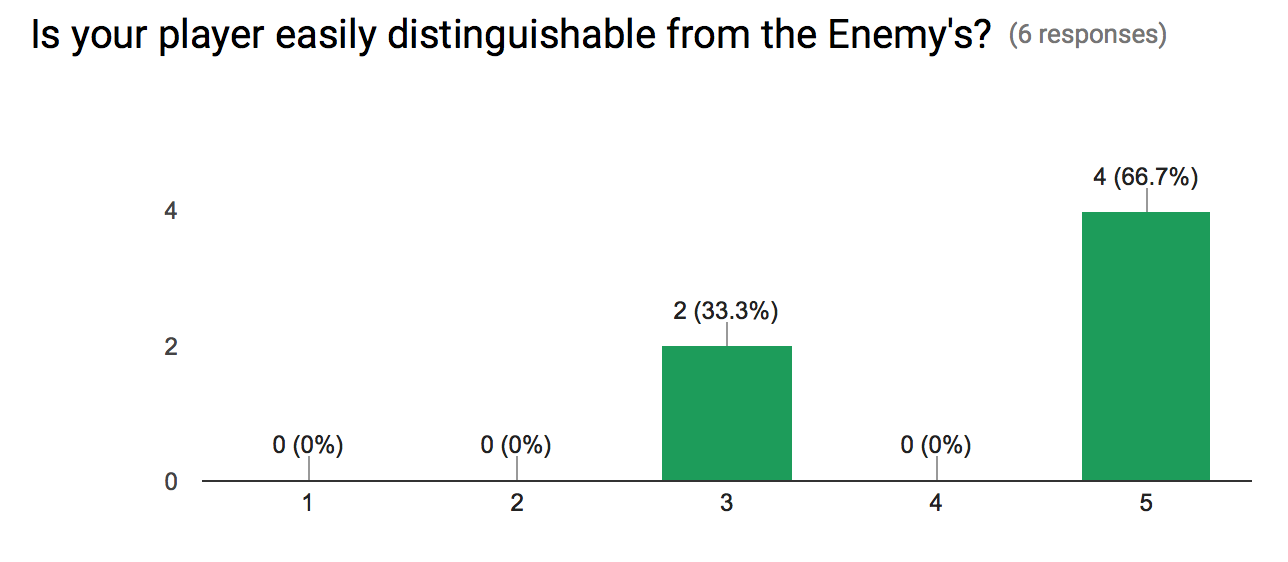
\includegraphics[width=\textwidth]{./Figures/1.png}
	\caption{Tank distinguishability Feedback}
\end{figure}
\item Can wooden walls be distinguished from Steel walls.
\begin{figure}[H]
	\centering
	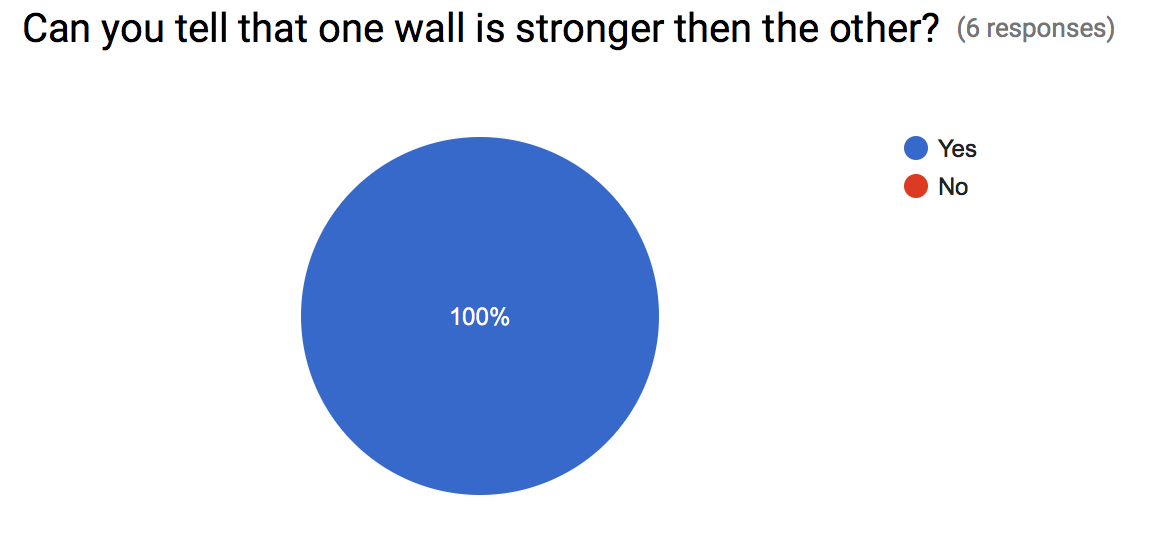
\includegraphics[width=\textwidth]{./Figures/4.png}
	\caption{Rate wall strength by material}
\end{figure}
\begin{figure}[H]
	\centering
	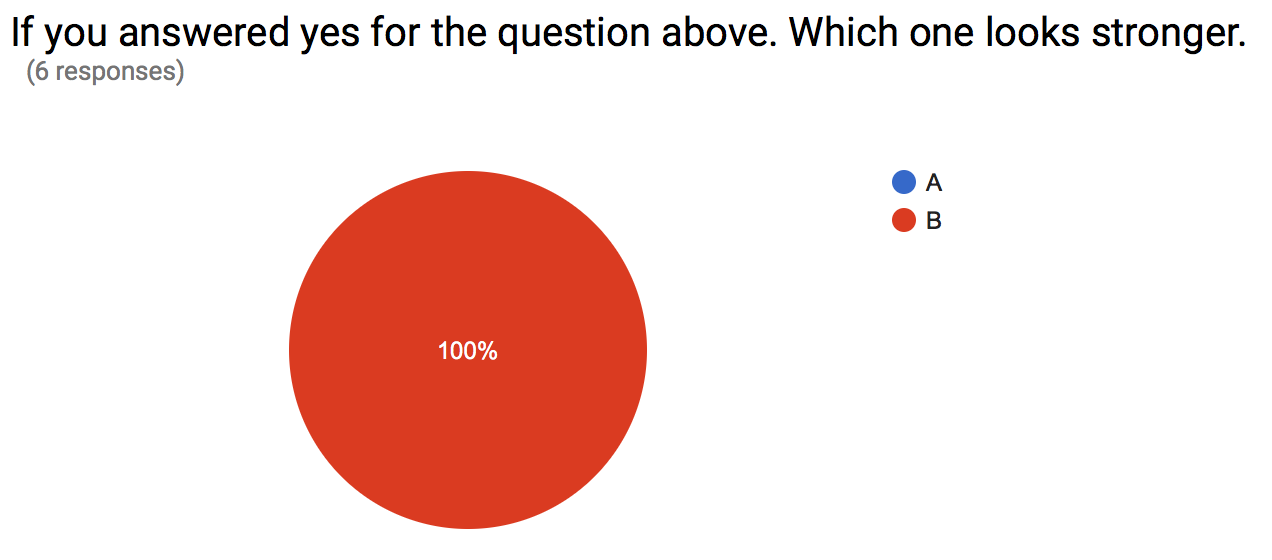
\includegraphics[width=\textwidth]{./Figures/6.png}
	\caption{Distinguish wall materials}
\end{figure}
\item Can the home base be distinguished
\begin{figure}[H]
	\centering
	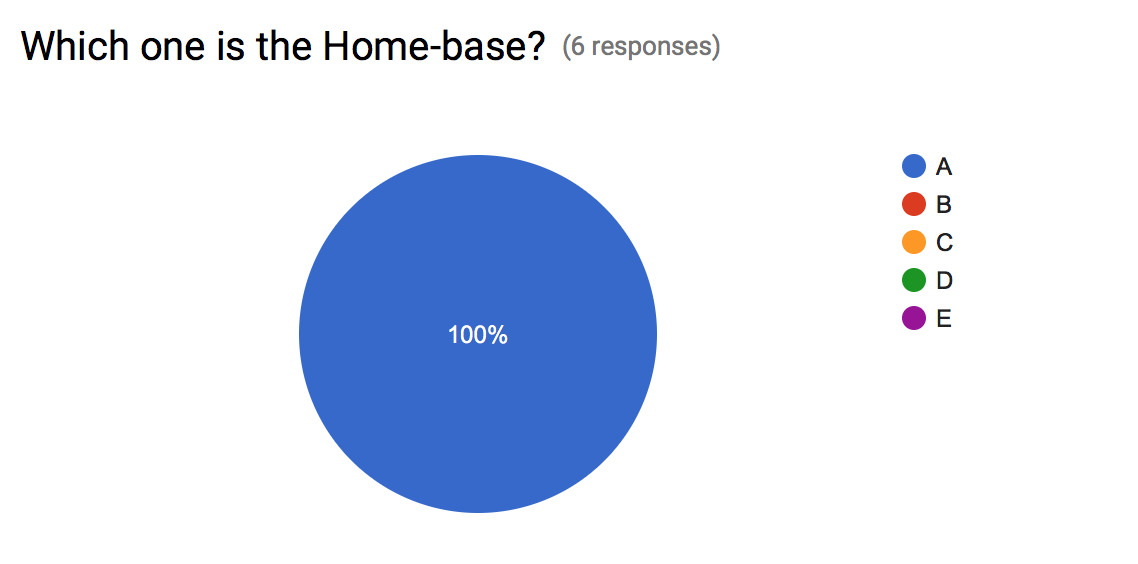
\includegraphics[width=\textwidth]{./Figures/3.png}
	\caption{Distinguish Home Base}
\end{figure}
\item Is the overall colour scheme is an eyesore.
\begin{figure}[H]
	\centering
	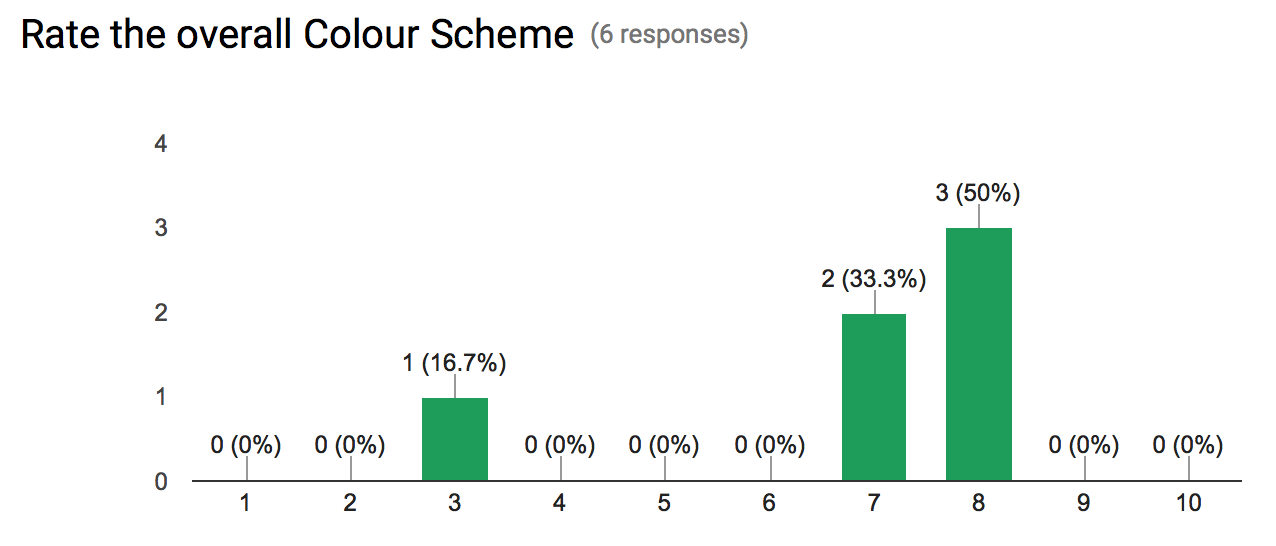
\includegraphics[width=\textwidth]{./Figures/7.png}
	\caption{Colour Scheme Feedback}
\end{figure}
\item Does the menu cover everything needed to play the game.
\end{itemize}
Pass:  If the game passes all manual unit tests on all browsers, the requirement
 is met.\newline
 \newline
Status: PASSED

\subsection{Ease of Use}
\label{sec:4.2}
Description: A survey will be provided to classmates whom will test the game 
and fill out the survey.  \newline
Questions: 
\begin{itemize}
\item Is the response time satisfying
\begin{figure}[H]
	\centering
	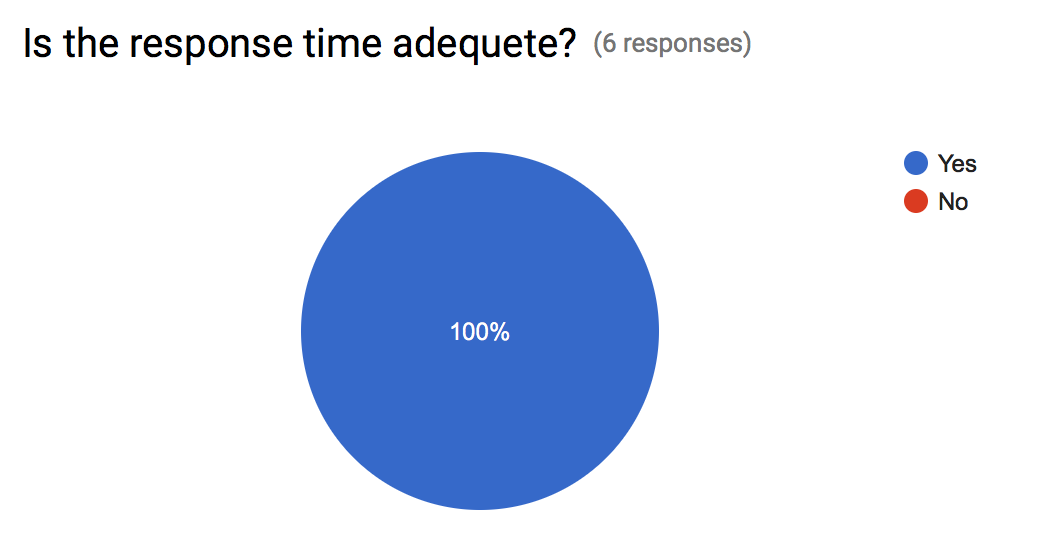
\includegraphics[width=\textwidth]{./Figures/13.png}
	\caption{Response Time Feedback}
\end{figure}
\item Is the game straight forward to play
\begin{figure}[H]
	\centering
	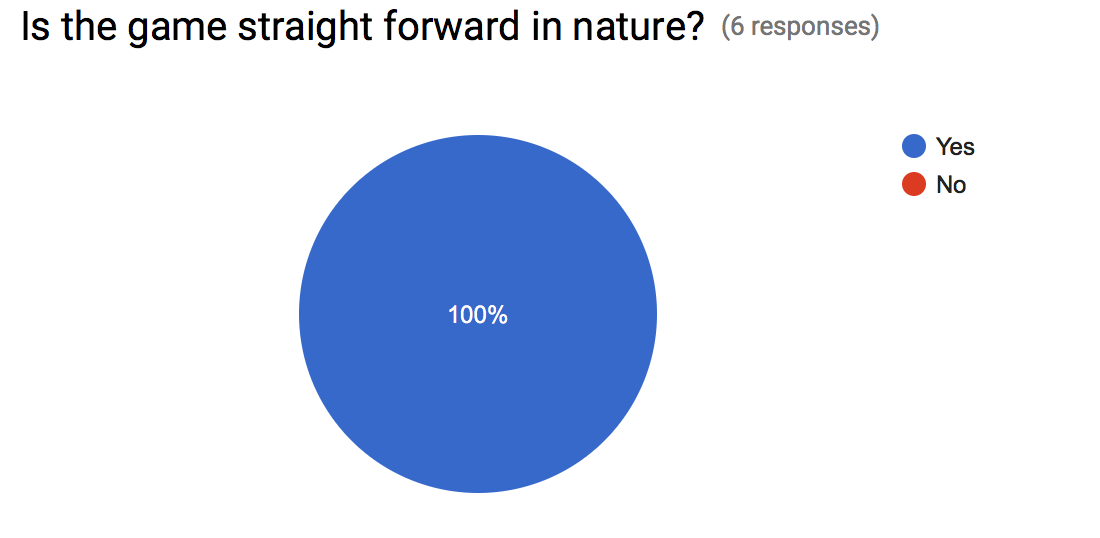
\includegraphics[width=\textwidth]{./Figures/14.png}
	\caption{Game Play Feedback}
\end{figure}
\item Are the instructions convoluted in nature.
\begin{figure}[H]
	\centering
	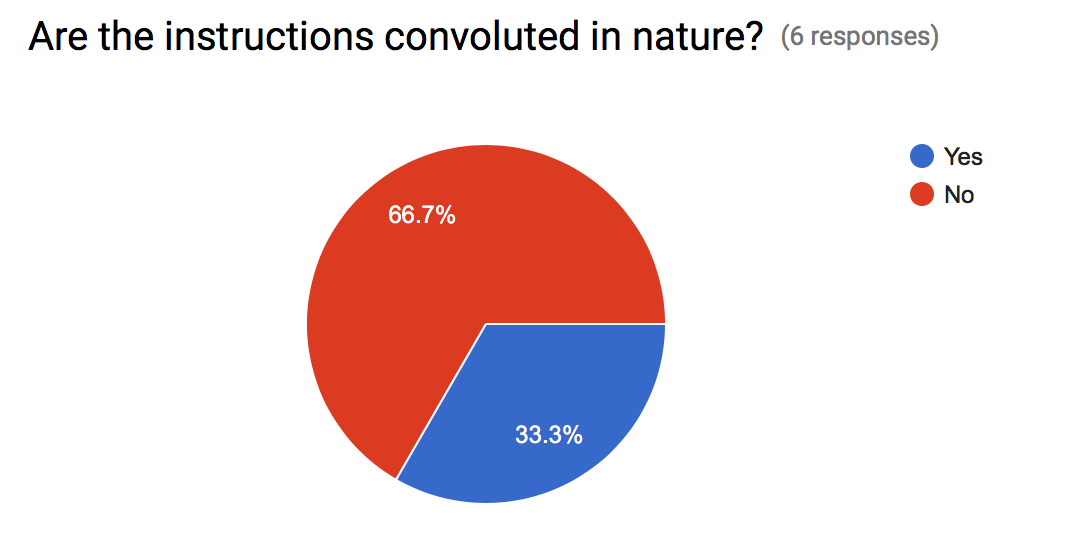
\includegraphics[width=\textwidth]{./Figures/16.png}
	\caption{Instructions Feedback}
\end{figure}
\item Are all menus understandable.
\begin{figure}[H]
	\centering
	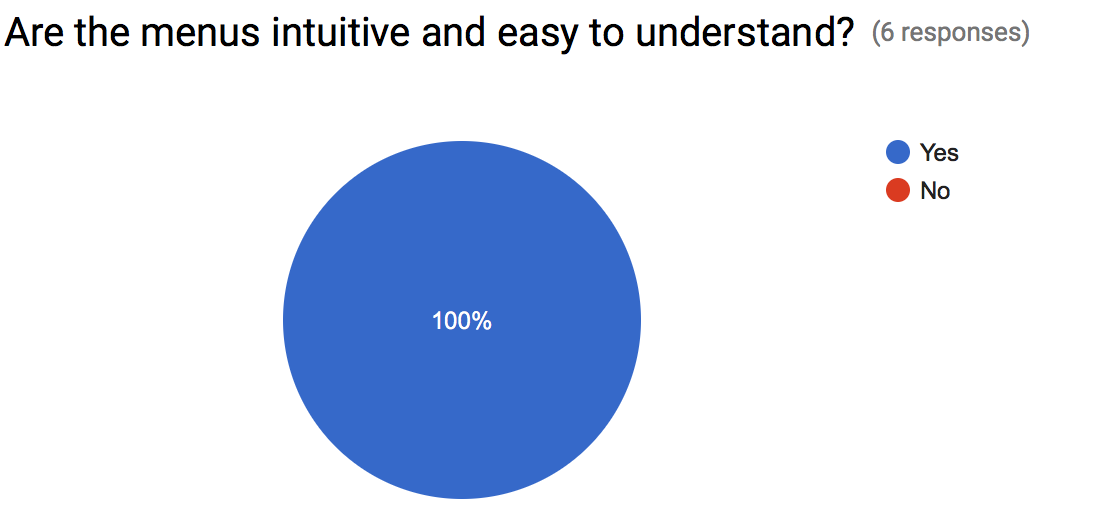
\includegraphics[width=\textwidth]{./Figures/15.png}
	\caption{Menu Feedback}
\end{figure}
\end{itemize}
Pass:  If the game passes all manual unit tests on all browsers, the requirement
 is met.\newline
 \newline
Status: PASSED


\subsection{Accessibility Requirements}
\label{sec:4.3}
Description: Test if the game functions on stated browsers.
How: running all manual unit tests from section 4.1 on the following browsers:
\begin{itemize}
\item Google Chrome
\item Mozilla Firefox
\item Apple Safari
\end{itemize}
\begin{figure}[H]
	\centering
	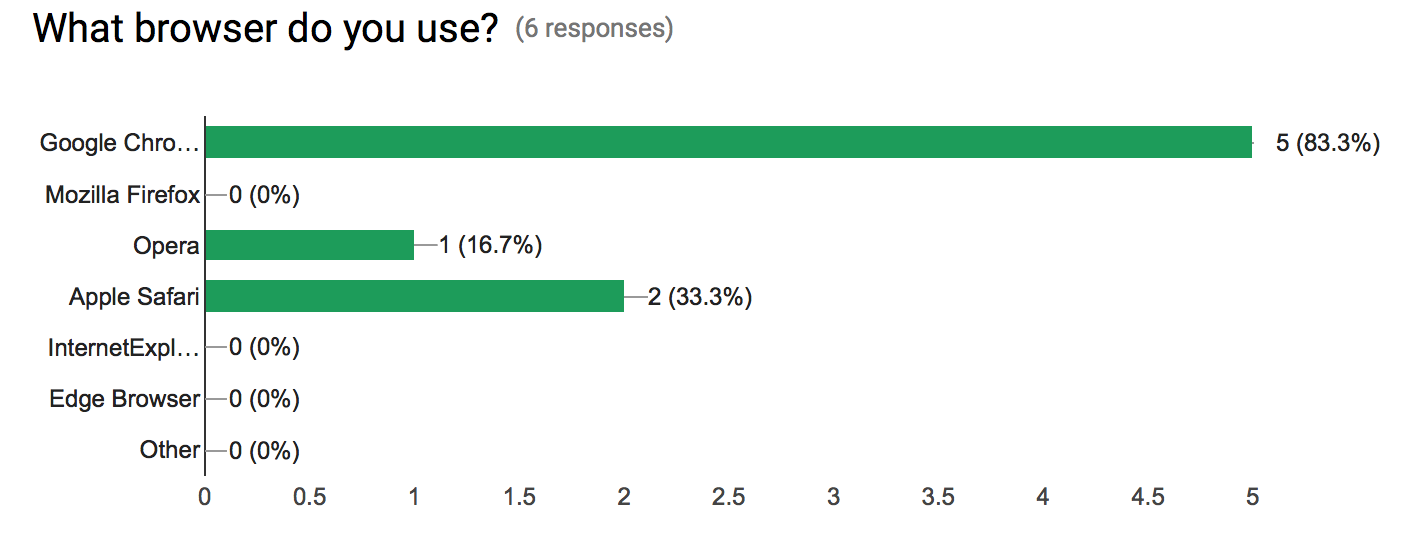
\includegraphics[width=\textwidth]{./Figures/9.png}
	\caption{Browsers Used}
\end{figure}

\begin{figure}[H]
	\centering
	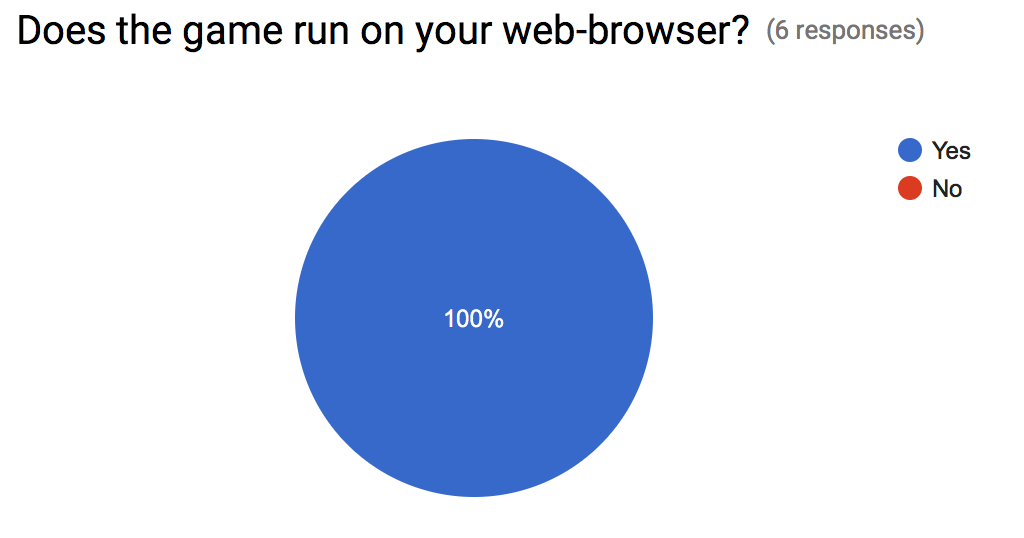
\includegraphics[width=\textwidth]{./Figures/8.png}
	\caption{Browsers Feedback}
\end{figure}
Pass:  If the game passes all manual unit tests on all browsers the requirement
 is met.\newline
 \newline
Status: PASSED

 \subsection{Performance}
 \label{sec:4.4}
Description: The game should run at an equal speed across all platforms and 
hardware specifications.  \newline
How: Playing a standard game on the following systems: 
\begin{itemize}
\item Late 2013 - MacBook Pro
\item Lab - Virtual Computer
\item Thode - Virtual Computer
\item 2014 - Surface Pro 3
\end{itemize}
\begin{figure}[H]
	\centering
	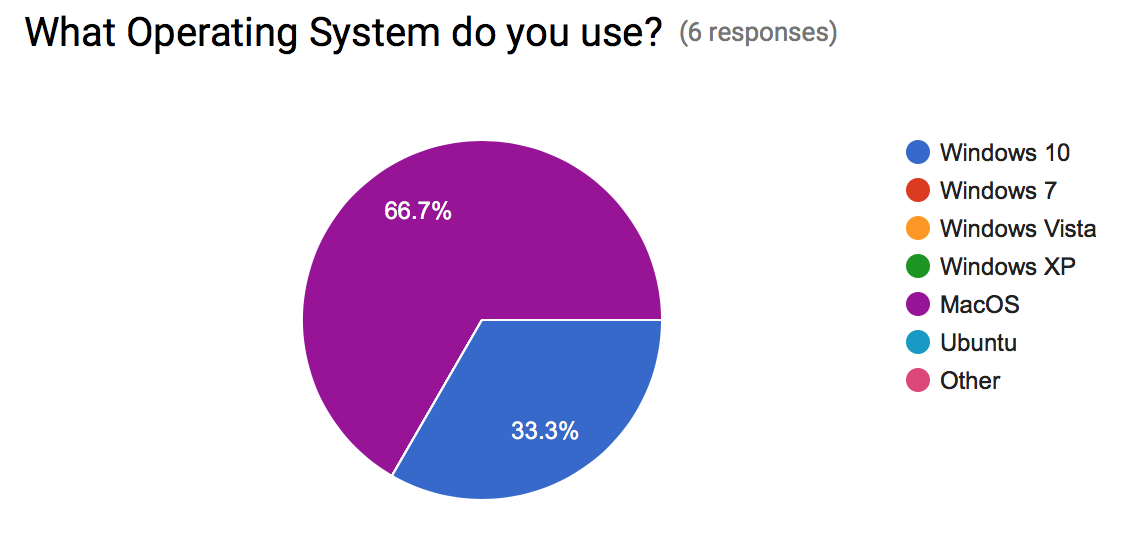
\includegraphics[width=\textwidth]{./Figures/10.png}
	\caption{Operating System Feedback}
\end{figure}
Pass: If game runs at similar speeds across all platforms, where relative 
similarity will be decided by tester.
\newline
 \newline
Status: PASSED


 \subsection{Maintainability}
 \label{sec:4.5}
 Description: The game's source code should be easy to read, maintain, and 
 learn from. \newline
 How: Have a classmate whom does not work with JS to read over an object file, 
 and have them tell us if they find the code easy to understand. \newline
 Pass: Classmate states that code is easy to read and learn from.
 \newline  \newline
Status: PASSED


 \subsection{Security}
 \label{sec:4.6}
Description: The game should not access and send user data to an external 
source \newline
How: Download the source files, then close all network connections.\newline
Pass: If the game is able to run off-line, it is not sending any data back.
Reasoning: If one method in JS fails the entire script usually crashes
\newline  \newline
Status: PASSED

\subsection{Legal Requirements}
\label{sec:4.7}
 Description: The game should follow Canadian Anti-Spam legislation \newline
 How: Review legislation and look through code to ensure legislation is 
 followed. \newline
 Pass: Legislation is not violated.
 \newline  \newline
Status: PASSED
 
\section{Comparison to Existing Implementation}
The open source game software we are working on is simply a Java application 
in its existent form. We are uploading the same game on a web browser which 
requires a different programming language altogether. As a result, we have not 
been able to use any existing code and have had to program the game completely 
from scratch. We have also not looked into the Java code to learn its 
implementation style or use any ideas for specific functions. Therefore, any 
similarities between our code and the existing code are coincidental. \\ \\
The major difference between the two implementations is that we have HTML, and 
CSS files in addition to the JavaScript source code which are required for any 
kind of web development. The existing code works with multiple classes 
representing different aspects of the game which can be seen in our code as 
well. However, it has more classes, three of them which are main method 
classes which can be explained by the programming language used. Our 
implementation has no main method or class, but instead the HTML file is used 
as the main class which drives the whole game. Another important difference is 
the style of programming; the existing implementation has made use of threads 
which we have not as we are still learning to work with JavaScript. The use of 
object oriented programming is evident in both implementations. For example, 
objects for tanks, bots, and barriers are included in both. 





%sections not relevant to product
%\subsection{Unit testing for output files}
%\section{Appendix}
%\subsection{Symbolic Parameters}



\end{document}